\documentclass[aspectratio=169,11pt,svgnames,draft]{beamer}

\usepackage[english]{babel}
\usepackage{graphicx}
\usepackage{enumitem}
\usepackage{amsmath}
\usepackage{mathtools}
\usepackage{float}
\usepackage{tikz}
\usetikzlibrary{patterns,arrows.meta}
\usepackage{tkz-euclide}
\tikzset{point style/.style = {%
  draw = black,
  inner sep = 0pt,
  shape = circle,
  minimum size = 5pt,
  fill = black
 }
}
\usepackage{pgfplots}
\pgfplotsset{compat=1.18}
\usepackage{pgf-pie}

\usepackage{enumitem}

\usepackage{caption}
\usepackage{subcaption}

% Flowchart stuff

\usepackage{pgfopts}
\usepackage{xcolor}
\usepackage{tcolorbox}

\usetheme[
 titlestyle=style2,
 titleformat=smallcaps,
 sectionstyle=plain,
 slidestyle=cyber,
 headingcolor=theme,
 block=transparent
]{trigon}

\title{Statistics}
\date{\today}
\author{Adam Klepáč}
\institute[GEVO]{Gymnázium Evolution Jižní Město}
\biglogo[width=.2\textwidth]{logo}
\smalllogo[width=.1\textwidth]{logo}
\titlegraphic{
\includegraphics[height=\paperheight]{title.jpg}}

\def\subsectionname{}

% enumerate global settings
\setlist[enumerate,1]{label=\arabic*.}
\setlist[enumerate,2]{label=\alph*)}

% custom colors %
\definecolor{MyTeal}{HTML}{64CCC5}
\definecolor{MyNavy}{HTML}{053B50}
\definecolor{MyBlue}{HTML}{176B87}
\definecolor{MyWhite}{HTML}{EEEEEE}
\colorlet{tPrim}{MyTeal}
\colorlet{tTheme}{MyTeal}
\colorlet{tSec}{MyNavy}
\colorlet{tAccent}{MyBlue}

\tcbset{
 boxsep=7pt,
 fonttitle=\sc,
 colframe=tGreyBg,
 colframe=tPrim,
 boxrule=1pt
}

\newcommand{\clt}{\textcolor{MyTeal}}
\newcommand{\cln}{\textcolor{MyNavy}}
\newcommand{\clb}{\textcolor{MyBlue}}
\newcommand{\clw}{\textcolor{MyWhite}}

\begin{document}
\titleframe

% \begin{frame}
%  \frametitle{What Even Is Statistics?}
%  \begin{tcolorbox}[title=Statistics]
%   \alert{Statistics} is a mathematical discipline concerned with predicting
%   future state of a system based \emph{solely} on its past behaviour.
%  \end{tcolorbox}
%  \pause
%  The collective information about a system's past state is called
%  \alert{data}.\\
%  \pause
%  It assigns \alert{probabilities} to each possible future state of system based
%  on data.\\
%  \pause
%  It also assigns probabilities to the \alert{possibility of wrong prediction}.
% \end{frame}
%
% \begin{frame}
%  \frametitle{Example -- Biased Coin?}
%  We throw a coin 10 times with the following outcome:
%  \[
%   \{H,H,H,T,H,T,H,H,H,T\},
%  \]
%  $H$ for `heads', $T$ for `tails'.
%  \pause
%  We can ask two questions:
%  \pause
%  \begin{itemize}[label=\textbullet]
%   \item<3-> What is the probability that the \alert{next toss} will come out
%    `heads'/`tails'?
%   \begin{itemize}[label=\textminus]
%    \item<5-> We got $7$ heads out of $10$ tosses, so the probability for the next toss
%     being heads is $7 / 10$.
%   \end{itemize}
%   \item<4-> Is this coin is \alert{biased towards} `heads'/`tails' with
%    \emph{allowed probability of error} $\alpha$?
%    \begin{itemize}[label=\textminus]
%     \item<6-> \alert{No}, for $\alpha = 0.05$.
%     \item<6-> \alert{Yes}, for $\alpha = 0.2$.
%    \end{itemize}
%  \end{itemize}
% \end{frame}
%
% \begin{frame}
%  \frametitle{Contents}
%  \tableofcontents
% \end{frame}
%
% \section{Data}
%
% \begin{frame}
%  \frametitle{What Do We Mean By Data?}
%  \begin{tcolorbox}[title=Data]
%   \alert{Two sets} (called \emph{inputs} and \emph{outputs}) describing the
%   studied system.
%  \end{tcolorbox}
% \end{frame}
%
% \begin{frame}
%  \frametitle{Example -- Junctions}
%  For a year, we keep track of the number of traffic accidents per day on road
%  junctions across the city to determine which should be first replaced by
%  roundabouts.\\
%  \pause
%  An \alert{input} is a day in a year.\\
%  \pause
%  An \alert{output} is the number of traffic accidents in a given day.
% \end{frame}
%
% \begin{frame}
%  \frametitle{Example -- First Baby}
%  We study the age that women bear children for the first time across Europe.\\
%  \pause
%  An \alert{input} would be a name of a European country.\\
%  An \alert{output} is the average age of a first-time mother in that country.
% \end{frame}
%
% \subsection{Types of Data}
%
% \begin{frame}
%  \subsectionpage
% \end{frame}
%
% \begin{frame}
%  \frametitle{Discrete Data vs. Continuous Data}
%  \begin{tcolorbox}[title=Discrete Data]
%   We call a data \alert{discrete} if the set of \emph{inputs} (and therefore also
%   that of \emph{outputs}) is \alert{countable}.
%  \end{tcolorbox}
%  \pause
%  Both previous examples feature \alert{discrete} data.
%  \begin{itemize}[label=\textbullet]
%   \item There are only \emph{finitely many} junctions in a city.
%   \pause
%   \item There are only \emph{finitely many} countries on a continent.
%  \end{itemize}
% \end{frame}
%
% \begin{frame}
%  \frametitle{Discrete Data vs. Continuous Data}
%  \begin{tcolorbox}[title=Continuous Data]
%   We call a data \alert{continuous} if the set of inputs is \alert{uncountable}.
%   In this case, the data is actually a \alert{function}: set of inputs $ \to $
%   set of outputs.
%  \end{tcolorbox}
%  \pause
%  More often than not, the inputs in a continuous data are \alert{moments in
%  time} or \alert{coordinates in space}.
% \end{frame}
%
% \begin{frame}
%  \frametitle{Continuous Data -- Examples}
%  \begin{itemize}[label=\textbullet]
%   \item We study the number of trains in a railway station at any given time.
%   \pause
%   \begin{itemize}[label=\textminus]
%    \item Input: time (of day);
%    \pause
%    \item Output: number of trains in the station.
%    \pause
%    \item The data is a function $f:[0,24] \to \mathbb{N}$.
%   \end{itemize}
%  \pause
%  \item Another example is the density of air per cubic meter.
%  \pause
%  \begin{itemize}[label=\textminus] 
%   \item Input: Coordinates of a unit cube in space.
%   \pause
%   \item Output: The combined weight of air molecules.
%   \pause
%   \item The data is a function $f:\mathbb{R}^3 \to \mathbb{R}$. 
%  \end{itemize}
%  \end{itemize}
% \end{frame}

\section{Visualizing Discrete Data}

\begin{frame}
 \frametitle{Pie Chart}
 Only usable if your outputs \alert{total a predetermined number}, typically
 \emph{percentages}.\\
 \pause
 Suppose we have three inputs --
 $\textcolor{VioletRed}{I_1},\textcolor{Aqua}{I_2}$ and
 $\textcolor{ForestGreen}{I_3}$ -- with three outputs --
 $\textcolor{VioletRed}{30 \%}, \textcolor{Aqua}{10 \%}$ and
 $\textcolor{ForestGreen}{60 \%}$.\\
 \pause
 Pie chart of this data looks like this
 \begin{center}
  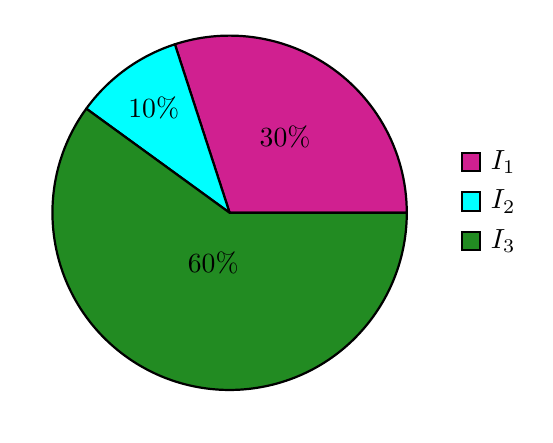
\begin{tikzpicture}[scale=0.75]
   \pie[color={VioletRed,Aqua,ForestGreen},text=legend]{
    30/$I_1$,
    10/$I_2$,
    60/$I_3$
   }
  \end{tikzpicture}
 \end{center}
\end{frame}

\begin{frame}
 \frametitle{Pie Chart -- Examples}
 Pie charts are frequently used to represent compositions of chemicals.\\
 \pause
 For instance, here is a pie chart of the composition of \emph{air}.
 \begin{center}
  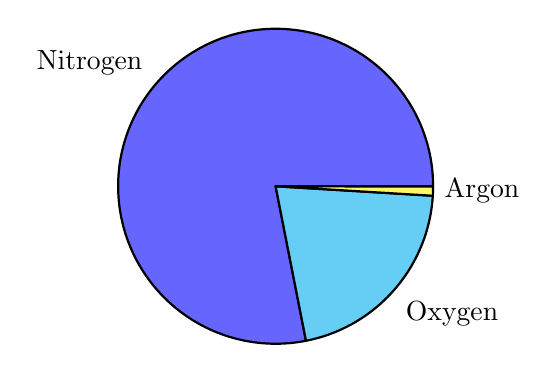
\begin{tikzpicture}
   \pie[hide number,radius=2]{
    78.09/Nitrogen,
    20.95/Oxygen,
    0.93/Argon
   }
  \end{tikzpicture}
 \end{center}
\end{frame}

\begin{frame}
 \frametitle{Pie Chart -- Examples}
 Favourite type of movie as determined by a survey.
 \begin{center}
  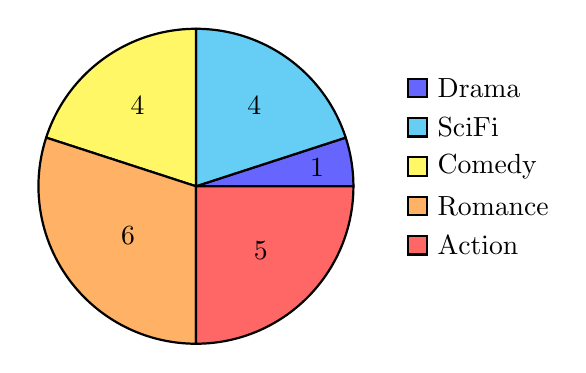
\begin{tikzpicture}
   \pie[radius=2,text=legend,before number=,after number=,sum=20]{
    1/Drama,
    4/SciFi,
    4/Comedy,
    6/Romance,
    5/Action
   }
  \end{tikzpicture}
 \end{center}
\end{frame}

\end{document}
